\documentclass[a4paper,oneside,article,11pt]{memoir}
\usepackage[english]{babel}
\usepackage[utf8]{inputenc}
\usepackage{amsmath,amssymb,amsthm}

% This font looks so good.
\usepackage[sc]{mathpazo}

% Typesetting pseudo-code
\usepackage{algorithm}
\usepackage{algorithmic}
\usepackage{multirow}
% Code comments like [CLRS]
\renewcommand{\algorithmiccomment}[1]{\makebox[5cm][l]{$\triangleright$ \textit{#1}}}
\usepackage{framed,graphicx,xcolor}
\usepackage[font={small,it}]{caption}
\usepackage{listings}
\usepackage{units}

% Relative references
\usepackage{varioref}

\usepackage{hyperref}

\bibliographystyle{plain}

\title{Advanced Data Structures \\ Project 2 - van Emde Boas Trees}
\author{Peter Gabrielsen 20114179 \\
Christoffer Hansen 20114637}
\newcounter{qcounter}
\begin{document}

\begin{titlingpage}
\clearpage

\maketitle
\thispagestyle{empty}

\begin{abstract}
missing
\\
\\
\\
The code can be found at: \\\url{Insert link to code here!}.
\end{abstract}
\end{titlingpage}

\pagebreak

\tableofcontents

\pagebreak

\chapter{Introduction}
van Emde Boas trees are interesting since they circumvent the sorting bound by restricting the keys in the data structure to be from $0$ to $n-1$ and with no duplicates similar to counting sort. With this restriction it allows the priority queue operations and some more in $\mathcal{O}(\log\log n)$ worst case time. In this project we will let our universe be 24-bit integer keys. We will run experiments that compare the van Emde Boas tree's priority queue operations to the binary heap~\cite{williams} and the Fibonacci heap~\cite{fred87}. Our findings can be found in section~\ref{chap:pqe}.

The van Emde Boas tree also supports finding the predecessor of an element in $\mathcal{O}(\log\log u)$ time which we will experimentally compare to the $\mathcal{O}(\log n)$ time of the Red-Black tree. We will also experimentally compare other tree operations for these two trees. The results of these experiment are found in section~\ref{chap:treee}
\chapter{Implementation}
\label{cpt:implementation}


\subsection{van Emde Boas tree}
The van Emde Boas tree was implemented as described in Introduction to Algorithms~\cite{clrs}. It is a non space-reduced tree and as such it will take time proportional to allocating the full universe of the tree in memory, to construct such a tree. However the tree will not grow in memory after allocation. A way to mitigate this, and thereby make the tree space-reduced would be to, instead of storing the complete structure, we should only store the substructures that actually contain elements. This could have been implemented by using hash maps instead of arrays.

Decrease key in the van Emde Boas tree was implemented as a delete and an insert giving an $\mathcal{O}(\log\log u)$ bound for this operation. The other asymptotic bounds for the van Emde Boas tree can be found in table~\ref{tab:van_emde_boas}.
\begin{figure}[H]
\begin{center}
\begin{tabular}{c|c}
Operation & Running time \\\hline
\texttt{FindMin} & $\mathcal{O}(1)$ \\\hline
\texttt{Insert} & $\mathcal{O}(\log\log u)$ \\\hline
\texttt{Delete} & $\mathcal{O}(\log\log u)$ \\\hline
\texttt{DeleteMin} & $\mathcal{O}(\log\log u)$ \\\hline
\texttt{PredecessorSearch} & $\mathcal{O}(\log\log u)$ \\\hline
\texttt{DecreaseKey} & $\mathcal{O}(\log\log u)$
\end{tabular}
\end{center}
\caption{Asymptotic running time for the van Emde Boas tree}
\label{tab:van_emde_boas}
\end{figure}

%TODO no page faults since we load everything in memory at beginning!

\subsection{Red-Black tree}
The Red-Black tree was implemented as described in Introduction to Algorithms~\cite{clrs}.

The Red-Black tree is a very popular balanced binary search tree and supports basic dynamic-set operations in time $\mathcal{O}(\log n)$.

\chapter{Experimental setup}
\label{chtp:experiment_setup}
%TODO write something about the machine which ran the experiments and something about how we measure the different things. Maybe copy all this from the AE report?

The experiments were performed on a machine with a Intel i5-3210M @ 2.5GHz (Ivy Bridge) with 128K bytes of L1 cache, 512K bytes of L2 and 3072K bytes of L3 cache. The machine had 4.2GB ram and ran Ubuntu 14.04 with kernel version 3.16.0-50.

The running time was measured using the built in \texttt{high\_resolution\_clock} in the \texttt{chrono} library. This measures the wall clock. It is the clock in \texttt{c++} with the highest precision, i.e. the shortest tick period.

The code is compiled with \texttt{g++ 4.8.4} with the \texttt{c++11} standard enabled and no optimization level.

The elements in our data structures were 32 bit integers. Random elements were generated uniformly in the 32 bit integer range using the Mersenne Twister 19937 from the \texttt{random} library.

CPU measurements were collected using \texttt{PAPI 5.3.0.0}

We used \texttt{perf} to measure page faults.

\chapter{Priority queue experiments}
\label{chap:pqe}
In this section we will design and perform experiments where we compare the van Emde Boas tree based priority queue with more standard priority queue implementations, namely the Fibonacci heap and binary heap. We will for each priority queue operation describe the experiments, present the results of said experiments and discuss those in detail.

\section{\texttt{FindMin}}
Finding the minimum in all three priority queues are constant time operations. They all just involve returning a stored element or dereferencing a pointer. We therefore expect to see all three queues perform similar and constant in the size of the input. In this experiment we do not measure running time since this is a constant time operation. Instead we measure the number of cycles and branch operations performed when calling find minimum in the respective queues. The experiments are repeated 10 times and averaged. The results are depicted in figure~\ref{fig:findmin_br} and~\ref{fig:findmin_cyc}.

\begin{figure}[H]
\centering
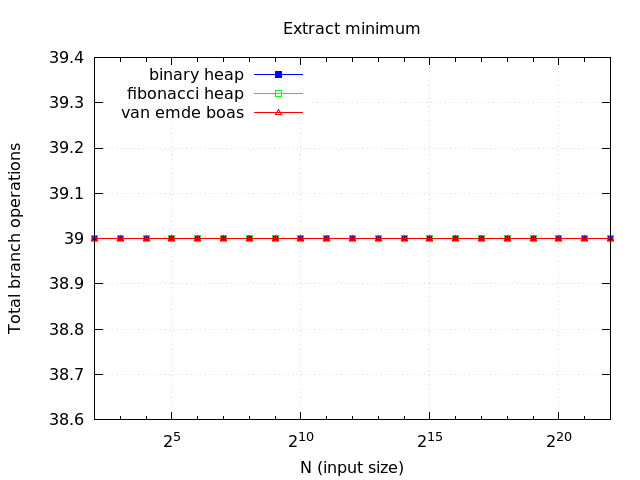
\includegraphics[scale=0.5]{../res2/findmin/extract_min_branch.png}
\caption{Number of branch operations for finding the minimum element}
\label{fig:findmin_br}
\end{figure}

\begin{figure}[H]
\centering
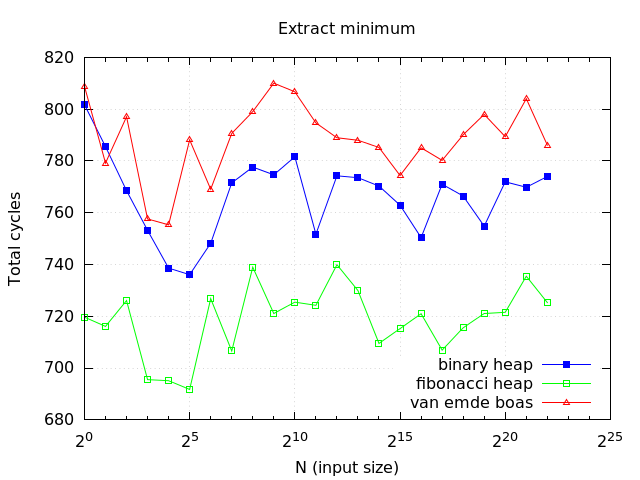
\includegraphics[scale=0.5]{../res2/findmin/extract_min_cycles.png}
\caption{Number of cycles for finding the minimum element}
\label{fig:findmin_cyc}
\end{figure}

The results clearly depict that finding the minimum does not depend on the input size and we conclude that the theoretical bound of $\mathcal{O}(1)$ also matches the experimental found results.

\section{\texttt{Insert}}
The asymptotic running times of the priority queues are as depicted in figure~\ref{fig:asymptotic_insert}.

\begin{figure}[H]
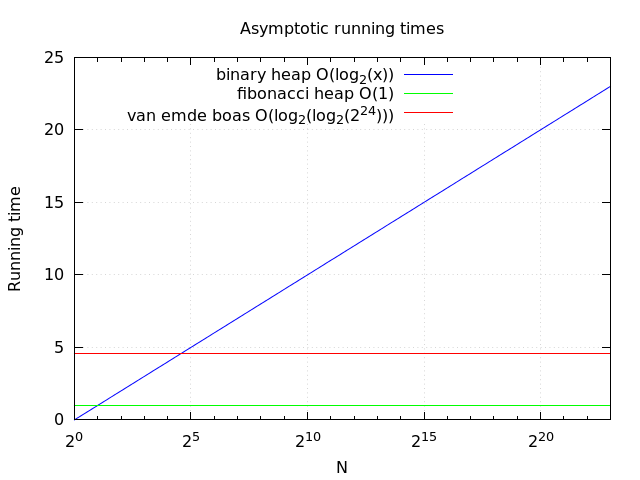
\includegraphics[scale=0.5]{../res2/inserts/runtime_plot.png}
\caption{Asymptotic running times for inserting in the priority queues.}
\label{fig:asymptotic_insert}
\end{figure}

We notice that inserting into the van Emde Boas tree does not depend on the size of the input but rather on the size of the universe that the tree hold. Since we support a universe of integers in the range from $0$ to $2^{24}$ we should have an insert that takes $\log\log 2^{24} = 4,5$ i.e. a larger constant than the Fibonacci heap but none the least a constant. What we expect to see in the worst case experiment is that the Fibonacci always performs best and at some point the van Emde Boas tree will outperform the Binary Heap with logarithmic asymptotic running time.

In order to see this result we remember from our previous experiments with priority queues that we need to experiment with the worst case data for the binary heap in order to see the logarithmic behaviour of the heap. This observation also makes it obvious that we do not want to see the behaviour of the heaps on random data since these would be similar to previous results from our first report. In figure~\ref{fig:insert_worst_running} we depict the results of running on the worst case data 10 times and averaging the result. The results confirm our hypothesis and that the running time of the van Emde Boas tree is independent of the input size while the binary heap is logarithmically dependent.

\begin{figure}[H]
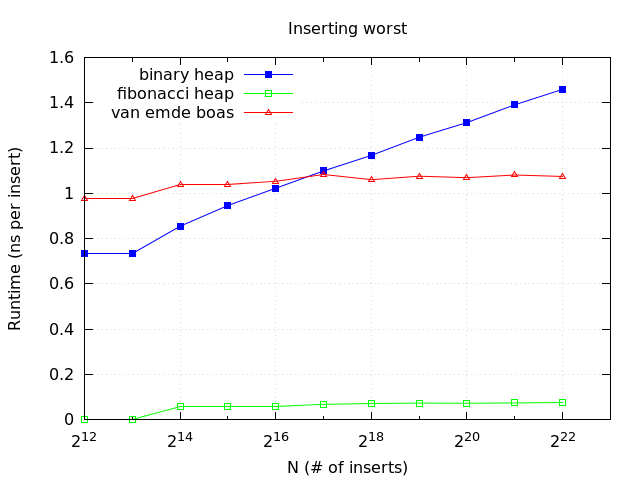
\includegraphics[scale=0.5]{../res2/inserts/runtime_worst.png}
\caption{Worst case running time for the priority queues.}
\label{fig:insert_worst_running}
\end{figure}

Looking at the number of branch operations in figure~\ref{fig:insert_worst_branch} we see that the number of branch operations is constant for the van Emde Boas tree and the Fibonacci heap while the binary heap increases logarithmically.

\begin{figure}[H]
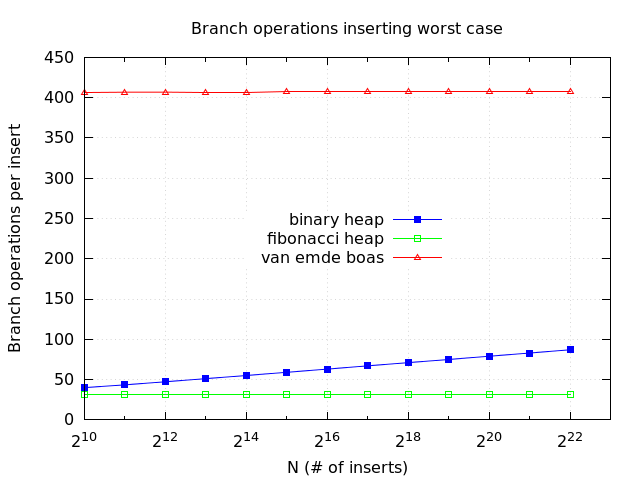
\includegraphics[scale=0.5]{../res2/inserts/branch_worst.png}
\caption{Worst case branching operations for the priority queues when inserting.}
\label{fig:insert_worst_branch}
\end{figure}


\section{\texttt{DeleteMin}}
Deleting the minimum element from a priority queue takes amortized logarithmic time for the Fibonacci heap. In the worst case it takes linear time if it is done after $n$ inserts due to the linear running time of consolidating the heap. The binary heap takes logarithmic time in the worst case since it might have to bubble the element all the way to the bottom again. The van Emde Boas tree deletes the minimum in $\mathcal{O}(\log\log u)$. In order to show these bounds experimentally we will make sure that the Fibonacci heap has consolidated and the binary heap operates in the worst case. The experiment will make two deletes to each priority queue and only measure the second. This way the Fibonacci queue has consolidated and we will only measure the amortized cost. The experiment was repeated 10 times and averaged. Since the operation is hard to measure using wall clock we measured the number of branching operations. The result of the experiment is depicted in figure~\ref{fig:insert_worst_branch}.

\begin{figure}[H]
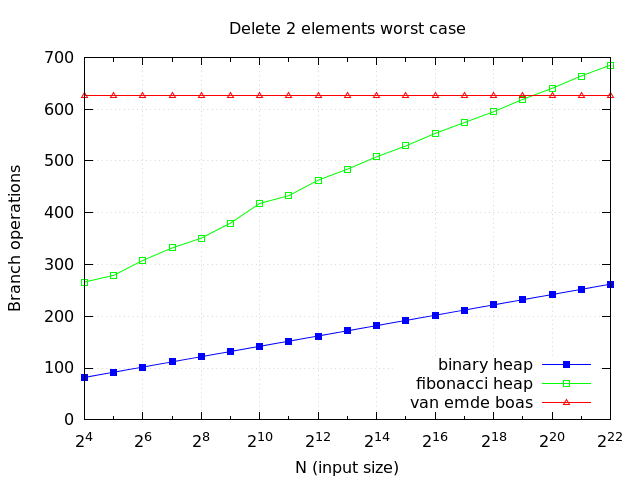
\includegraphics[scale=0.5]{../res2/delmin/delmin_del_2_branch_worst.png}
\caption{Worst case branching operations for the priority queues on delete minimum.}
\label{fig:insert_worst_branch}
\end{figure}

Figure~\ref{fig:insert_worst_branch} shows that both the binary heap and the Fibonacci heap are logarithmic in the input size while van Emde Boas remains constant in the input size as hypothesized.

\section{\texttt{DecreaseKey}}
Decreasing the key in the Fibonacci heap is an amortized constant time operation. The binary heap is logarithmic in the worst case and finally the van Emde Boas tree is as usual $\mathcal{O}(\log\log u)$. We implemented decrease key as an erase and an insert in the van Emde Boas tree.

The experiment tests the interesting worst case behaviour where we in the binary heap decrease the maximum element such that it has to bubble all the way to the top every time. The experiment first consolidates the Fibonacci heap and then runs 1 decrease key operation for various input sizes. The result are depicted in figure~\ref{fig:dk_worst_1}.

\begin{figure}[H]
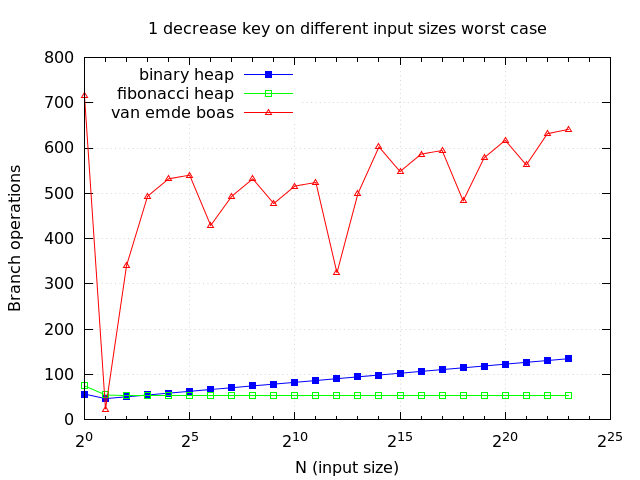
\includegraphics[scale=0.5]{../res2/dk/dk_worst_1.png}
\caption{Worst case branching operations for the priority queues on decrease key.}
\label{fig:dk_worst_1}
\end{figure}


\section{Conclusion}
Finding the minimum element took constant time for all three priority queue implementation as expected.

Insert was found to be a constant time operation for the Fibonacci heap, a $\mathcal{O}(\log\log u)$ time operation for the van Emde Boas tree, and finally a logarithmic time operation for the binary heap in the worst case.

Deleting the minimum element was found to be a constant time operation for the van Emde Boas tree, while is a logarithmic time operation for the binary heap and Fibonacci heap.

Finally decrease key was found to be constant for the Fibonacci heap, logarithmic for the binary heap and %TODO what about van emde boas

\chapter{Red-Black tree \& van Emde Boas}
\label{chap:treee}

\chapter{Conclusion}


\bibliography{references}

\end{document}


